\newpage

% Из текста короткого задания на ВКР:
% 1. Определение средств разработки и архитектуры системы: разработка ее структуры;
% 2. определение набора необходимого оборудования, программного обеспечения.

% 3. Проектирование и определение спецификаций аппаратной и программной компонентов системы.
% 4. Реализация компонентов системы с использованием выбранных средств разработки.
% 5. Сборка макета аппаратной подсистемы.
% 6. Сборка, установка и тестирование программного обеспечения аппаратной и программных подсистем.
% 7. Тестирования системы, интеграции программной и аппаратных частей.

\section{Разработка программно-аппаратной системы}

В данном разделе описывается проектирование аппаратной части системы~--- считывателя бесконтактных платежных карт~--- и разработка программной части СБО~--- программного обеспечения для считывателя и мобильного приложение бесконтактной оплаты.
Для этого в соответствии с техническим заданием (ТЗ) решаются следующие задачи:

\begin{itemize}
    \item определение средств разработки и архитектуры системы: разработка ее структуры; определение набора необходимого оборудования, программного обеспечения;
    \item проектирование компонентов и определение спецификаций аппаратной части СБО, сборка макета аппаратной части системы;
    \item выбор архитектуры и подхода разработки программной подсистемы, проектирование программных компонентов СБО (программы мобильного терминала бесконтактной оплаты и мобильного приложения оплаты) и определение спецификаций компонентов;
    \item реализация компонентов системы с использованием выбранных средств разработки;
    \item сборка, установка и тестирование программного обеспечения аппаратной подсистемы и программного обеспечения программной подсистемы.
\end{itemize}

Разрабатываемая система является mPOS-терминалом с поддержкой бесконтактной оплаты.
Как любой mPOS-терминал она состоит из мобильного устройства и считывателя платежных карт, подключаемого к ней.
В соответствии с требованиями ТЗ считыватель поддерживает только бесконтактные карты и подключается беспроводным образов посредством технологии Bluetooth.
Считыватель взаимодействует с платежным средством посредством технологии NFC.

Процесс оплаты с использованием устройства представляет следующую последовательность действия:
\begin{enumerate}
    \item представить торгово-сервисного предприятия (ТСП) вводит данные о платеже в мобильное приложение и активирует считыватель;
    \item держатель карты прикладывает к считывателю средства платежа (карта или мобильное приложение, эмулирующее платежную карту);
    \item считыватель взаимодействует со средством платежа и передает данные, необходимые для формирования платежа, на мобильное устройство;
    \item мобильное устройство отправляет HTTP-запрос на сервер банка-эквайера для выполнения платежа;
    \item сервер банка-эквайера отправляет HTTP-ответ на мобильное устройство, сообщая о статусе операции.
\end{enumerate}

Плательщик (держатель карты) может убрать средство платежа от считывателя после того как считыватель выполнит все необходимые операции для получения данных, необходимых для формирования платежа, либо сообщит о невозможности продолжения транзакции из-за ошибок совместимости или выполнения взаимодействия.


\subsection{Разработка структуры системы}

Структура разрабатываемой системы представлена на рисунке~\ref{fig:struct_scheme}.
Направления стрелок показывают направления обмена данными между программными и аппаратными модулями.

\begin{figure}[H]
    \centering
    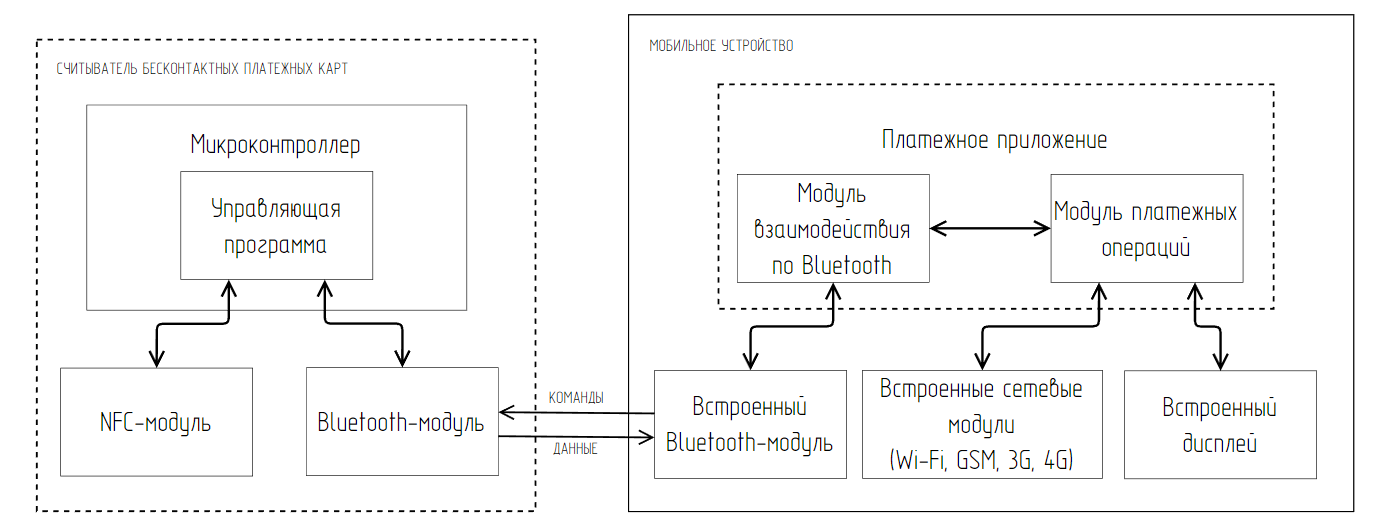
\includegraphics[width=0.8\textwidth]{images/design/struct_scheme}
    \caption{\centering Структурная схема системы}
    \label{fig:struct_scheme}
\end{figure}

Считыватель бесконтактных платежных карт включает в себя 3 аппаратных модуля в соответствии с требованиями ТЗ:
\begin{itemize}
    \item Bluetooth-модуль для связи с мобильным устройством, которое осуществляет выполнения платежных операций;
    \item NFC-модуль для взаимодействия с бесконтактной средством платежа;
    \item микроконтроллер для осуществления управления устройством (контроля работы NFC-модуля и Bluetooth-модуля).
\end{itemize}

Для микроконтроллера реализуется ПО, с помощью которого осуществляется управления NFC и Bluetooth модулями, через предоставляемые модулями интерфейсы для управления, описанных в их документации (форматом управляющих команд).
NFC-модуль подключается посредством разъема SPI, Bluetooth-модуль подключается посредством разъема USART для передачи управляющих команд с необходимыми данными.


Мобильное приложение включает в себя следующие программные модули:
\begin{itemize}
    \item модуль взаимодействия с устройством считывателем по Bluetooth,
    \item модуль платежных операций для сетевых запросов к API банка-эквайера.
\end{itemize}

Используются следующие аппаратные модули мобильного устройства:
\begin{itemize}
    \item Bluetooth-модуль для взаимодействия со считывателем,
    \item встроенные сетевые модули (Wi-Fi, GSM, 3G, 4G) для взаимодействия с сервером банка-эквайера,
    \item дисплей для взаимодействия с пользователем.
\end{itemize}

Структурная схема с внешними участниками процесса оплаты представлена на рисунке~\ref{fig:struct_scheme_out}.
На ней также указаны направления обмена данными между программными, аппаратными модулями и внешними участниками процесса оплаты.

\begin{figure}[H]
    \centering
    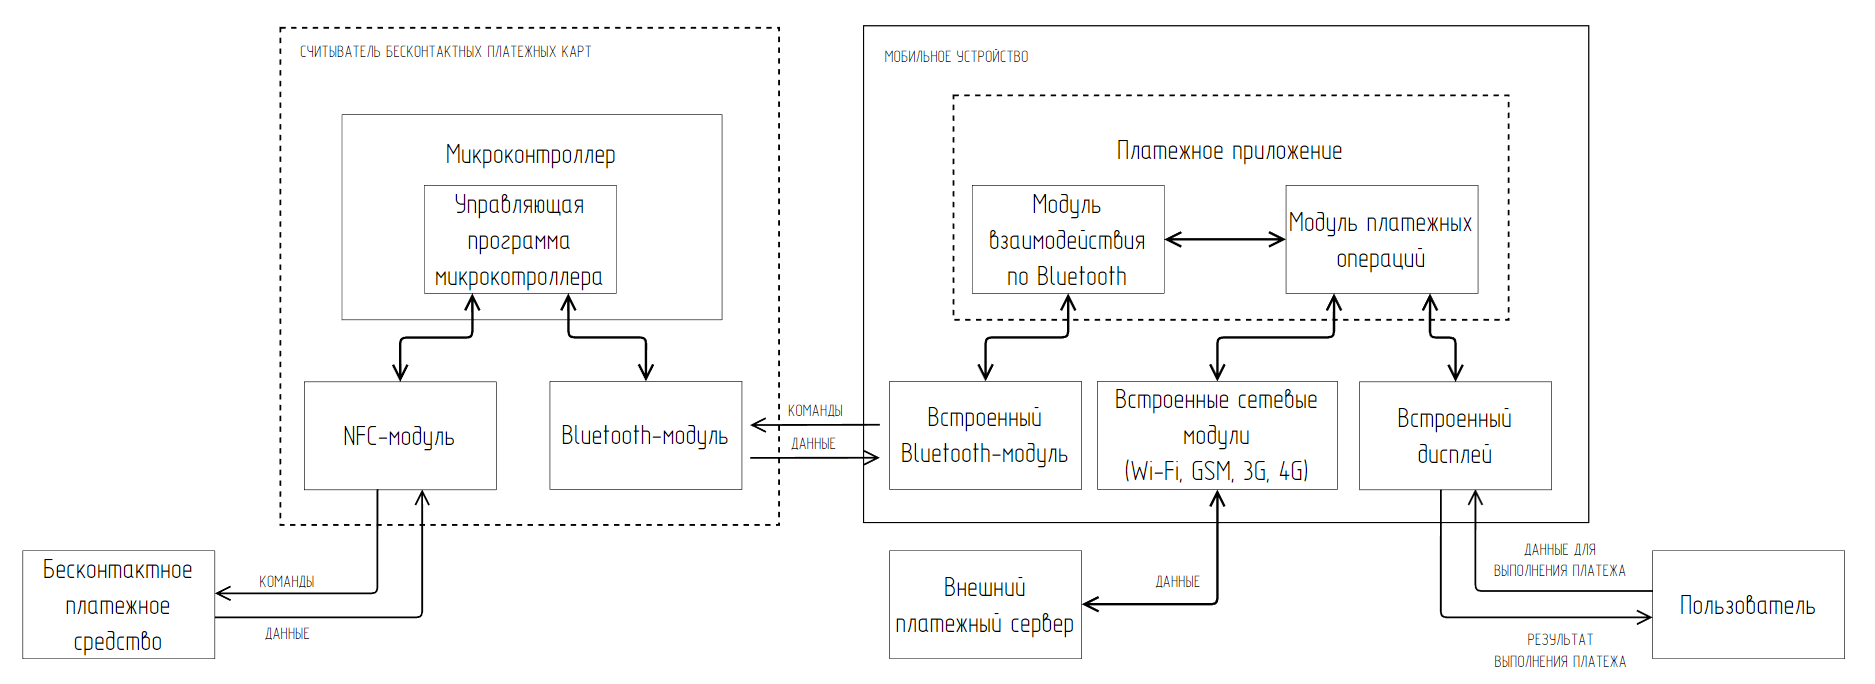
\includegraphics[width=0.8\textwidth]{images/design/struct_scheme_out}
    \caption{\centering Структурная схема системы с внешними участниками процесса оплаты}
    \label{fig:struct_scheme_out}
\end{figure}


\subsection{Разработка аппаратной части системы}

\subsubsection{Функциональная схема аппаратной части системы}

В соответствии с требованиями технического задания основные функции аппаратной части системы (микроконтроллерной системы):
\begin{itemize}
    \item взаимодействие со средством платежа посредством технологии NFC в соответствии со стандартом взаимодействия с бесконтактными средсвами платежа EMV Contactless, рассмотренном в исследовательской части;
    \item связь с мобильным устройством посредством технологии Bluetooth (получение управляющих команд и отправка полученных данных).
\end{itemize}

В данном процессе задействуется МК, Bluetooth-модуль и NFC-модуль.
Все эти компоненты работают как единая система под управлением МК.

% TODO нарисовать схему работы (диаграмму последовательностей)
Алгоритм работы устройства:
\begin{enumerate}
    \item настройка Bluetooth-модуля для подключения к мобильному устройству;
    \item установка соединения мобильного устройства и Bluetooth-модуля;
    \item получение команды от мобильного устройства о начале транзакции и суммы транзакции;
    \item включение и базовая настройка NFC-модуля микроконтроллером, начало поиска средства платежа;
    \item обнаружение средства платежа, установка соединения и взаимодействие с ним в соответствии алгоритмом представленном на рисунке~\ref{fig:kernel_transaction_flow}; % TODO: нарисовать mir_transaction и заменить
    \item передача полученных данных от средства платежа на мобильное устройство посредством Bluetooth;
\end{enumerate}

Структурная схема устройства представлена на рисунке~\ref{fig:apparat_struct}.
На ней NFC-модуль имеет детализированное изображение с целью демонстрации комплексности структуры данного устройства.

\begin{figure}[H]
    \centering
    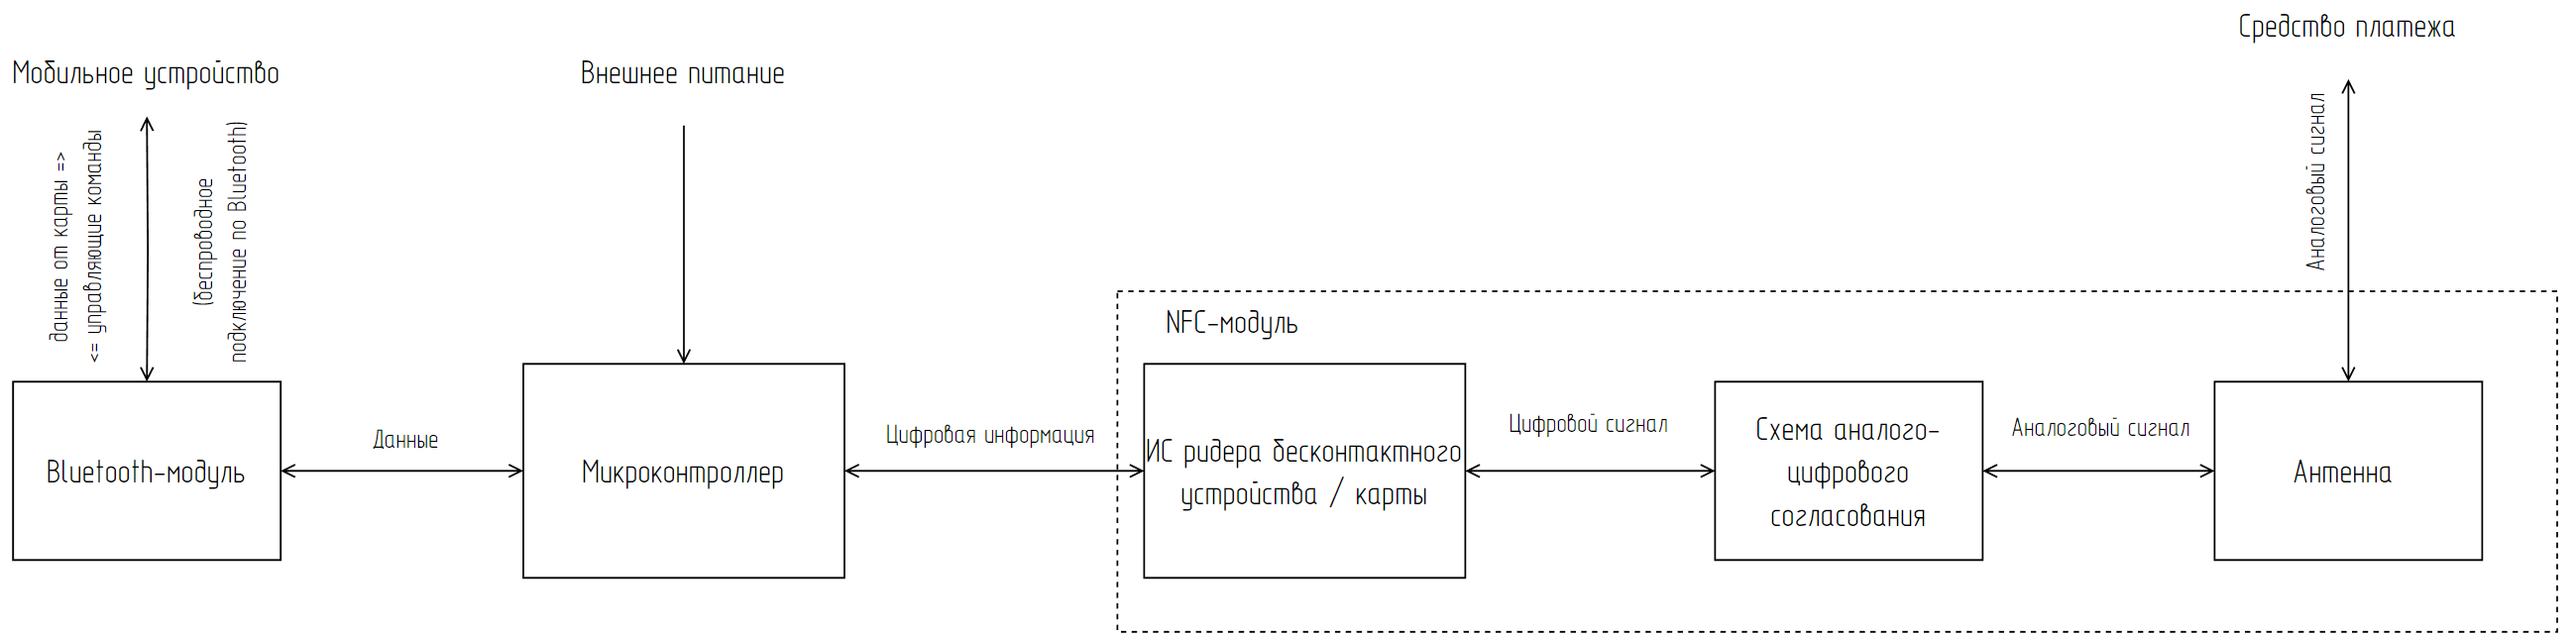
\includegraphics[width=0.8\textwidth]{images/design/apparat_struct}
    \caption{\centering Структурная схема считывателя бесконтактных платежных карт}
    \label{fig:apparat_struct}
\end{figure}


Согласно требованию ТЗ разрабатываемое устройство должно обеспечивать возможность подключения по Bluetooth к мобильному устройству, с возможностью приема и передачи данных, также оно должно взаимодействовать с бесконтактным средством платежа в соответствии со стандартом ISO/IEC 14443 с помощью модуля NFC, поддерживающему работу с картами ПС <<МИР>>.
Данные модули должны работать под управлением МК, имеющего разъемы SPI и USART для их подключения.
При этом стандарта EMV Contactless вводит строгие временные ограничения на время прямого непосредственного взаимодействия с картой (не более 0.4 мс).
Из чего следует, что МК должен обладать высокой производительностью.
ISO/IEC 14443-A используемый в платежных картах обладает скоростью передачи данных 106 кбит/с или 13.25 кбайт/с, что с учетом используемого компактного формата TLV для передаваемых сообщений и их размера, который значительно меньше чем объем, предаваемый даже за 1 мс, не создает ограничений по производительности.

При анализе существующих mPOS-терминалов было установлено, что они используют микропроцессоры с архитектурой Advanced RISC Machines (ARM), в частности ARM 7, ARM 9, ARM 11, которые обладают частотой более 100 МГц.
С учетом того, что данные терминалы используются для обработки транзакций различных платежных систем и не только бесконтактным образом для разрабатываемой системы данные процессоры будут избыточны, однако использование ARM архитектуры было бы крайне желательно.

В таблице~\ref{tab:microcontroller_comparison} приведены характеристики различных микроконтроллеров от разных компаний~\cite{stm32f103_datasheet}\cite{atmega328p_datasheet}.

\begin{longtable}[l]{|
P{0.18\textwidth}|
P{0.2\textwidth}|
P{0.15\textwidth}|
P{0.13\textwidth}|
P{0.2\textwidth}|}

    \caption{Сравнение характеристик часто используемых микроконтроллеров}
    \label{tab:microcontroller_comparison} \\
    \hline
    \textbf{Характеристика} &
    \textbf{ATmega328P} &
    \textbf{ESP8266} &
    \textbf{PIC16F8} &
    \textbf{STM32F103} \\
    \hline
    \endfirsthead

    \caption*{Продолжение таблицы~\ref{tab:microcontroller_comparison}} \\
    \hline
    \textbf{Характеристика} &
    \textbf{ATmega328P} &
    \textbf{ESP8266} &
    \textbf{PIC16F8} &
    \textbf{STM32F103} \\
    \hline
    \endhead

    \hline
    \endfoot

    \hline
    \endlastfoot

    Разрядность процессора &
    8 бит &
    32 бит &
    8 бит &
    32 бит \\
    \hline

    Тактовая частота &
    до 20 МГц &
    до 160 МГц &
    до 20 МГц &
    до 72 МГц \\
    \hline

    Флэш-память &
    32 КБ &
    4 МБ &
    14 КБ &
    64 КБ \\
    \hline

    SRAM &
    2 КБ &
    160 КБ &
    368 Б &
    20 КБ \\
    \hline

    EEPROM &
    1 КБ &
    Нет &
    256 Б &
    Нет \\
    \hline

    Количество I/O портов &
    23 &
    11 &
    13 &
    37 \\
    \hline

    Поддержка Wi-Fi &
    Нет &
    Да &
    Нет &
    Нет \\
    \hline

    Поддержка Bluetooth &
    Нет &
    Нет &
    Нет &
    Нет \\
    \hline

    Энергопотребление &
    Низкое &
    Среднее &
    Среднее &
    Низкое \\
    \hline

    Стоимость &
    Низкая &
    Низкая &
    Низкая &
    Низкая \\
    \hline
\end{longtable}

В ходе выполнения курсовой работы по дисциплине <<Микропроцессорные системы>> выбор был сделан в пользу микроконтроллера ATmega328P в составе платы Arduino Uno R3.
Данный вариант был удобен при первоначальном макетировании системы и изучении стандартов взаимодействия бесконтактной карты.
Однако частота данного МК значительно ниже чем у аналогов, у него 8-битная гарвардская архитектура процессора, при прочих равных Flash-памяти, SRAM, количество I/O-портов меньше чем у STM32F103.
Поэтому в качестве МК для аппаратной части системы используется STM32F103C8T6 на базе микропроцессора ARM Cortex-M3 с 32-битной архитектурой.
Данная архитектура позволяет работать с 32-битными регистрами, выполнять сложные математические операции, включая работу с плавающей запятой (с помощью программных или аппаратных средств).
Поддержка современных продвинутых программных библиотек, таких как HAL (Hardware Abstraction Layer), LL (Low Layer) и CMSIS (Cortex Microcontroller Software Interface Standard), предоставляет разработчику полный контроль над аппаратной частью микроконтроллера, с пониманием происходящих процессов на уровне регистров и таймеров.
В то же время, использование ATmega328P с Arduino.h для аналогичных задач часто приводит к неэффективному использованию ресурсов, ограничению функциональности и снижению производительности.
Кроме того, экосистема STM32 предоставляет мощные инструменты разработки, такие как STM32CubeIDE, которые упрощают настройку периферии и генерацию кода, сохраняя при этом гибкость и контроль над аппаратными ресурсами.

Для реализации беспроводного Bluetooth-соединения был выбран Bluetooth-модуль HC-05, обладающий следующими характеристиками:

\begin{itemize}
    \item напряжение питания: 3,3 В – 5 В;
    \item потребляемый ток: при подключении – до 40 мА (поиск, сопряжение, подключение), при передаче данных – до 8 мА;
    \item частотный диапазон: 2,4 ГГц – 2,48 ГГц;
    \item мощность передатчика: до +4 дБм;
    \item чувствительность приемника: 80 дБм;
    \item дальность связи: до 10 метров;
    \item интерфейс: UART (с последовательной передачей данных);
    \item поддерживаемые скорости передачи данных: 9600, 19200, 38400, 57600, 115200, 230400 и 460800 бит/сек;
    \item режимы работы: Master (ведущий) и Slave (ведомый);
    \item рабочая температура: от -25 °C до +75 °C;
    \item размеры: 27 x 13 x 2,2 мм~\cite{hc05_datasheet}.
\end{itemize}

HC-05 имеет дальность связи до 10 метров, поддерживает скорости передачи данных до 460800 бит/сек и может работать как в режиме Master (ведущий), так и в режиме Slave (ведомый).
Единственным недостатком является не самая актуальная версия технологии Bluetooth 2.0.
Однако даже модуль HC-08 имеет версию 4.0 (актуальная~-- 6.0) при стоимости в 4--5 раз выше.
Т.к. осуществляется процедура передачи данных без необходимости частого и многоразового подключения устройства-хоста к bluetooth-модулю, а приоритетом является низкое энергопотребление – стандарт Bluetooth 2.0 является преимуществом, а не недостатком.

Модуль HC-05 можно настроить с помощью AT-команд, которые отправляются через интерфейс USART.
Это позволяет изменить имя устройства, пароль для подключения, скорость передачи данных и другие параметры.
Примеры AT-команд:

\begin{itemize}
    \item AT – проверка связи с модулем;
    \item AT+NAME=NewName – изменение имени модуля;
    \item AT+UART=9600 – установка скорости передачи данных на 9600 бод.
\end{itemize}

Модуль HC-05 включает в себя чип BC417143 и работает на напряжении 5 В и реализуя прием и передачу сигнала.


Среди прочих NFC-модулей наиболее популярными являются модули компании NXP.
К тому они имеют качественную и исчерпывающую документацию.
NXP поставляет не только NFC-модули, но и микроконтроллеры с интегрированными модулями NFC, а также разрабатывает ПО для работы с модулями, однако только для МК собственного производства.

В качестве модуля для считывателя используется NXP PN5180.
Данный модуль имеет поддержку большого числа стандартов технологии NFC.
Имеет сравнительно низкую стоимость (порядка 700--1000 рублей на ноябрь 2024 года).
А также имеет широкий функционал и подробную документацию.
PN5180 является широко распространенным модулем, с поддержкой множества стандартов (в том числе и используемого в платежах~-- ISO14443-A).
Альтернативой ему могут выступать схожие модули от компании NXP, в частности PN5190 (улучшенная версия PN5180), однако он умеет выше стоимость и при этом улучшения в производительности и поддержки стандартов пренебрежимо малы в рамках данного устройства.

%Основные внутренние компоненты интегральной схемы модуля представлены на рисунке~\ref{fig:pn5180_components}~\cite{pn5180_datasheet}.
%
%\begin{figure}[H]
%    \centering
%    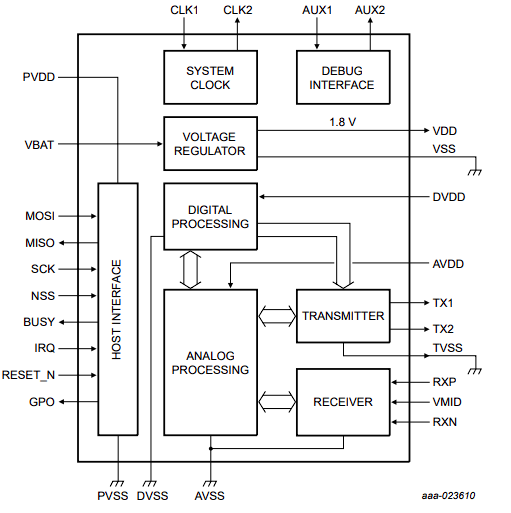
\includegraphics[width=0.8\textwidth]{images/design/pn5180_components}
%    \caption{\centering Компоненты интегральной схемы модуля PN5180}
%    \label{fig:pn5180_components}
%\end{figure}

Важно отметить, что производитель модуля предварительно выполняет следующие действия по его настройке:
\begin{itemize}
    \item определение целевого импеданса для оптимизации мощности RF-выхода и минимизации потребление энергии;
    \item проектирование EMC-фильтра для подавления нежелательных гармоник тока, которые могут создавать помехи в работе устройств;
    \item измерение LCR-параметров антенны (индуктивности, емкости и сопротивления) для работы;
    \item расчет компонентов для согласования антенны с NFC-модулем.
\end{itemize}

Также производится симуляция работы антенны, тестирование работы в реальных условиях и корректировка РЧ контура.
В результате чего получается надежный и стабильно работающий модуль, для которого нет необходимости в выполнении данных затруднительных действий, требующих дополнительного оборудования и навыков.


PN5180 использует для связи с микроконтроллером SPI, расширенный линией BUSY, что позволяет ему указыать о невозможности приема и отправки данных в конкретный момент времени.
Максимальная скорость его разъема SPI составляет 7 Мбит/с, при этом параметры SPI устанавливаются следующим образом: CPOL=0, CPHA=0 (SPI Mode 0), старший бит первым (MSB first).
На модуль по SPI передаются управляющие команды, список которых приведен в его datasheet в разделе <<Работа модуля NFC>>, с помощью этих команд происходит настройка модуля\cite{pn5180_datasheet}.

Уровень напряжения сигналов, которыми оперирует модуль, составляет 1,8--3,3 В.
У STM32F103C8T6 рабочий уровень напряжения на разъемах~--- 3.3 В, что делает его совместимым с данным модулем.
В свою очередь на разъемах микроконтроллера ATmega328P рабочим уровнем напряжения является 5 В, что усложняло его использование в первом разработанном макете устройства (возникала необходимость использования конвертера уровня напряжения, что повышало потрбляемую МК-системой мощность).


На функциональной схеме изображены используемые компоненты, необходимые для работы устройства.
Она показывает логическое соединение устройств, используемые для подключения контакты, а также направление передачи данных и управляющих сигналов между компонентами.
Спроектированная функциональная схема разработанного устройства представлена на рисунке~\ref{fig:func_scheme}, а также в приложении В.
У МК изображены только используемые компоненты.

\begin{figure}[H]
    \centering
    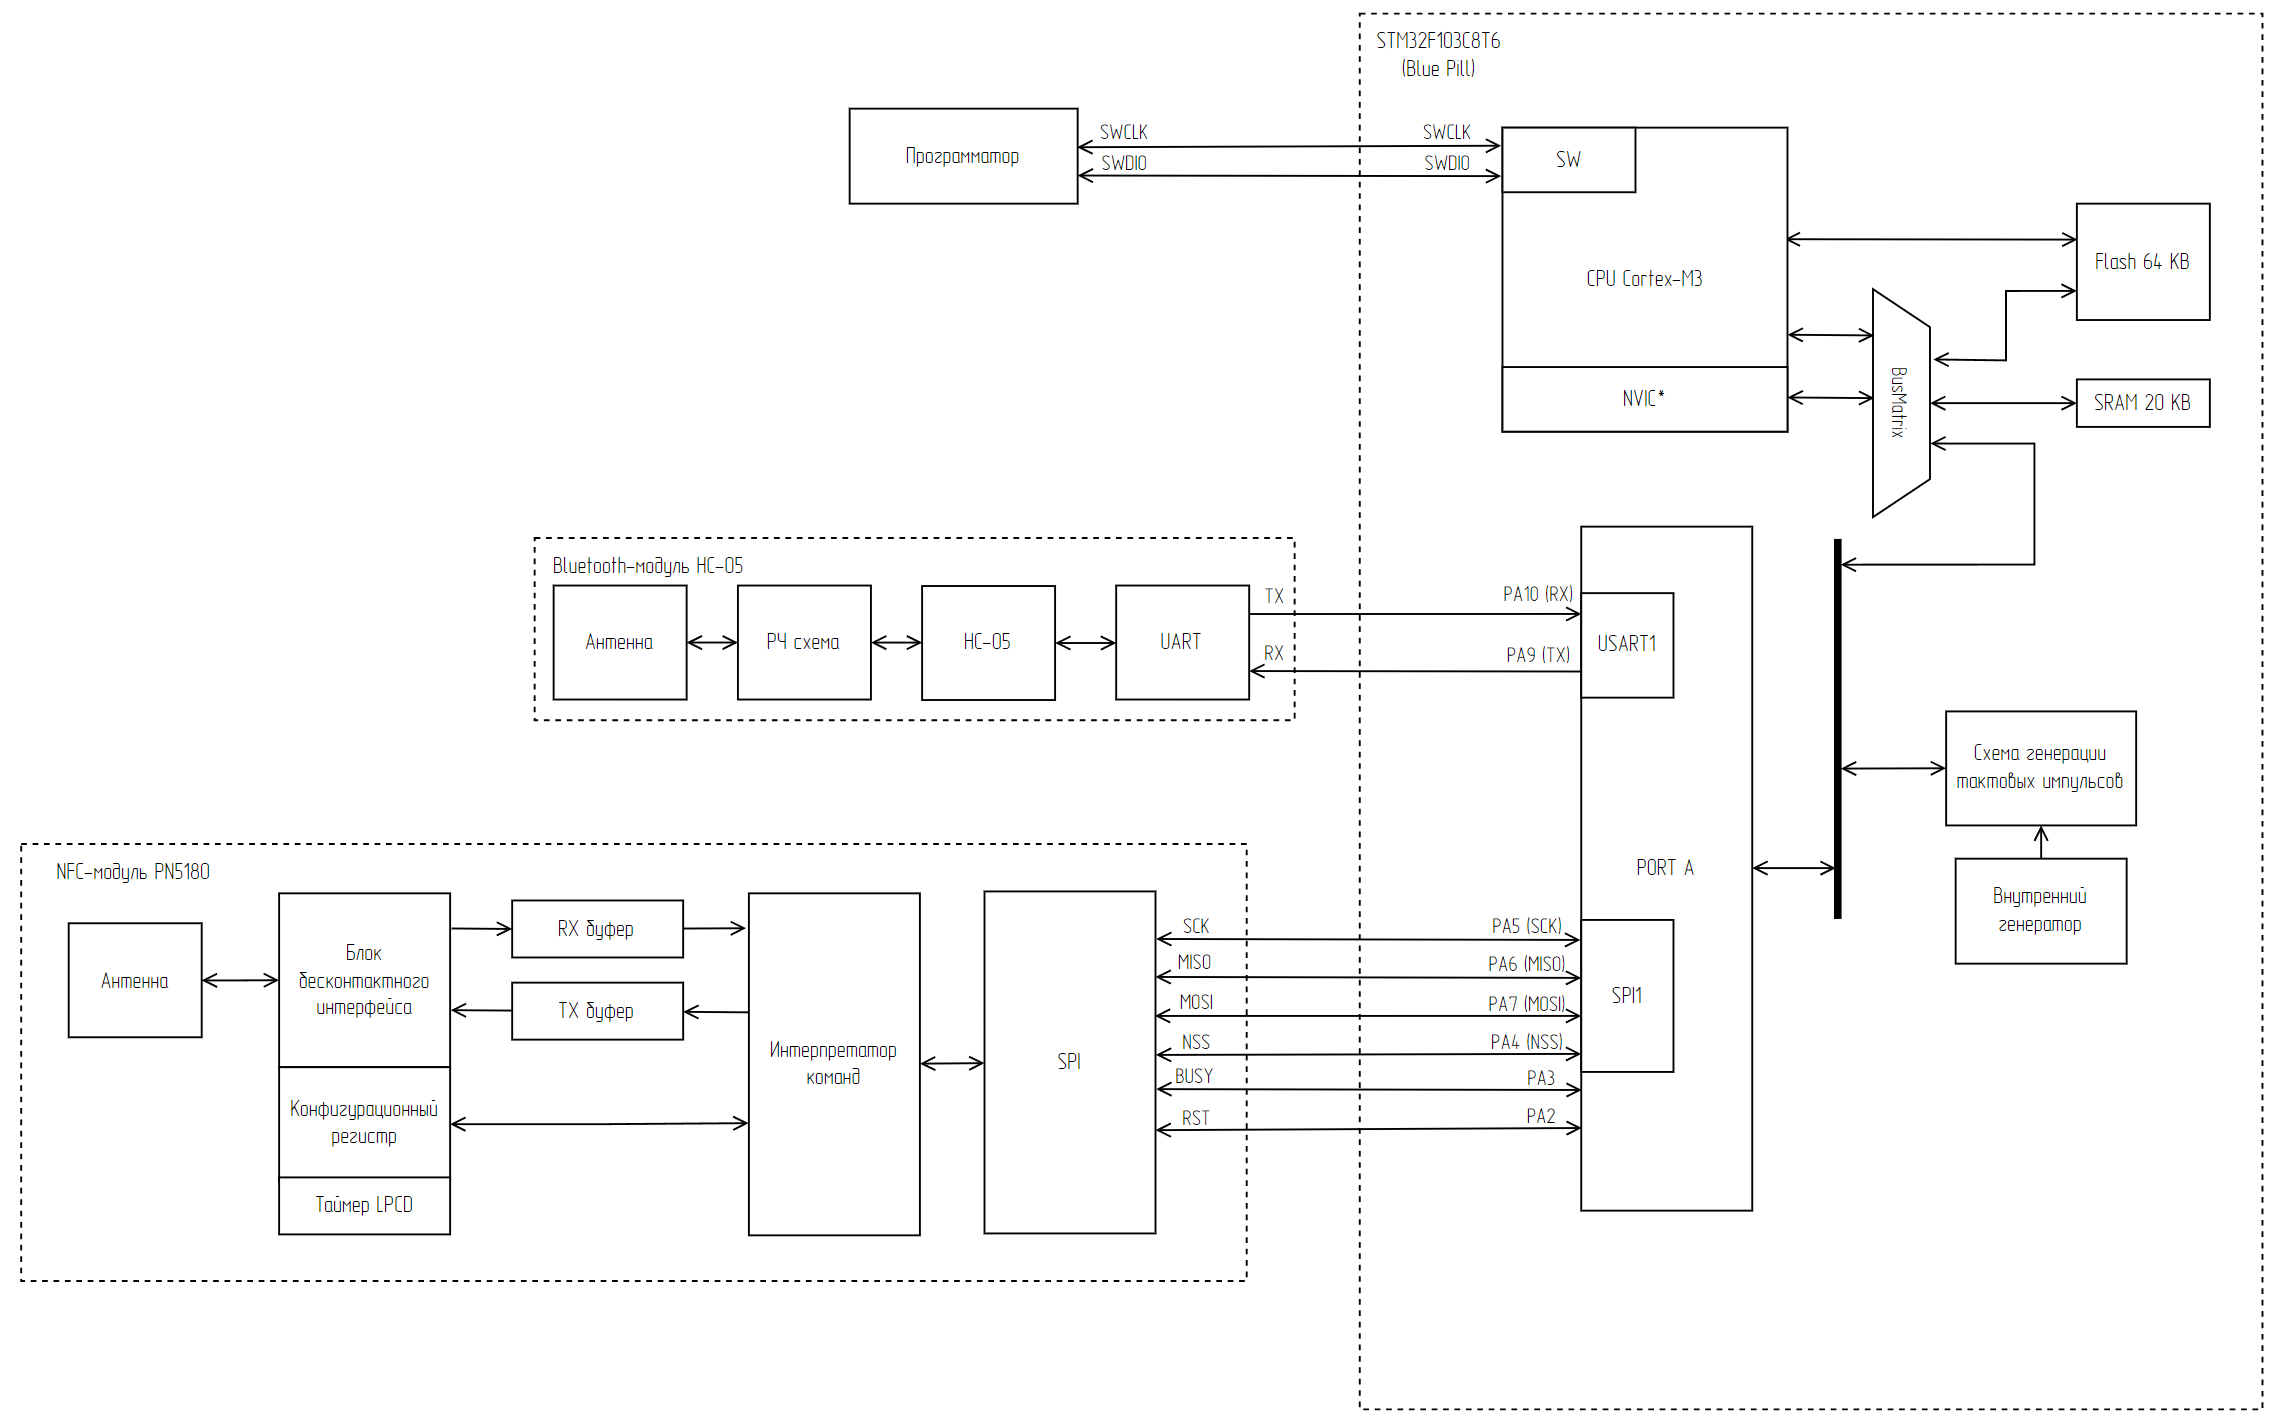
\includegraphics[width=1\textwidth]{images/design/func_scheme}
    \caption{\centering Функциональная схема считывателя бесконтактных платежных карт}
    \label{fig:func_scheme}
\end{figure}





\subsubsection{Принципиальная схема аппаратной части системы}

%\paragraph{Программирование МК}

Программирование микроконтроллера STM32F103C8T6 осуществляется с использованием интерфейса SWD (Serial Wire Debug), который является стандартным решением для отладки и прошивки большинства 32-битных ARM-микроконтроллеров.
Интерфейс SWD разработан для упрощенного подключения к микроконтроллеру, в отличие от JTAG, он использует минимальное количество выводов, что делает его особенно удобным в условиях ограниченного пространства на плате.

Для работы с этим интерфейсом необходимы всего два сигнальных контакта:
\begin{itemize}
    \item SWCLK — тактовая линия;
    \item SWDIO — двунаправленная линия передачи данных.
\end{itemize}

Также требуются линии питания и земли:
\begin{itemize}
    \item VCC — питание 3.3 В;
    \item GND — общий провод.
\end{itemize}

Процесс программирования выглядит следующим образом:

\begin{enumerate}
    \item программатор ST-Link v2 подключается к микроконтроллеру через разъем, соответствующий интерфейсу SWD;
    \item программатор устанавливает связь с ядром микроконтроллера, отправляя тактовые сигналы по линии SWCLK и управляя данными через SWDIO;
    \item происходит загрузка и запись кода во флэш-память микроконтроллера;
    \item МК автоматически перезапускается для исполнения загруженную программы.
\end{enumerate}

Таким образом, для программирования микроконтроллера STM32F103C8T6 через ST-Link v2 используется разъем SWD, представленный на рисунке~\ref{fig:swd}.

\begin{figure}[H]
    \centering
    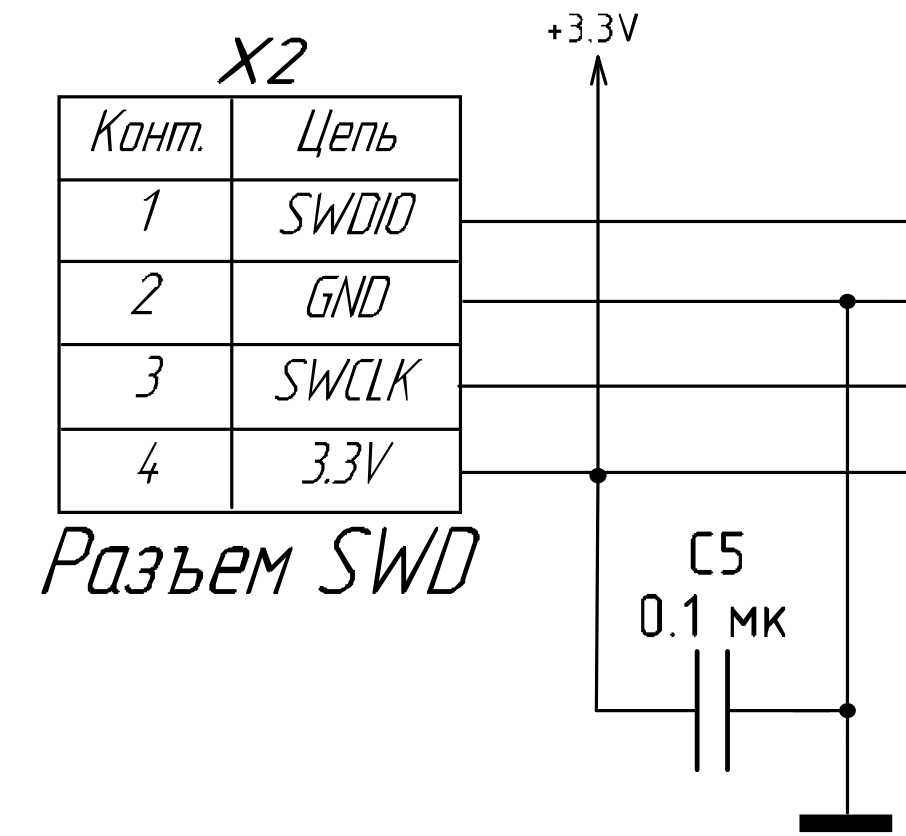
\includegraphics[width=0.4\textwidth]{images/design/swd}
    \caption{\centering Разъем программирования МК}
    \label{fig:swd}
\end{figure}

%\paragraph{Подключение цепи питания}

Для обеспечения работоспособности устройства необходимо подавать стабилизированное напряжение на микроконтроллер и прочие компоненты схемы.
В данной МК-систем питание микроконтроллера STM32F103C8T6 осуществляется через стандартный USB-разъём microUSB, который используется как интерфейс подключения к внешнему источнику питания.
Это позволяет отказаться от использования дополнительного внешнего источника питания и упрощает конструкцию устройства.
Разъем представлен на рисунке~\ref{fig:usb}.

\begin{figure}[H]
    \centering
    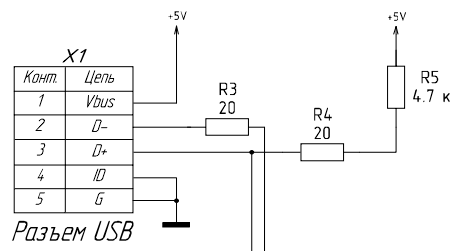
\includegraphics[width=0.4\textwidth]{images/design/usb}
    \caption{\centering Разъем питания МК}
    \label{fig:usb}
\end{figure}

Напряжение с USB поступает непосредственно на стабилизатор напряжения RT9193--33, т.к. микроконтроллер STM32F103C8T6 работает на напряжении 3.3 В, а не 5 В, как это часто бывает в других МК.
Стабилизатор преобразует напряжение с USB (5 В) к необходимому уровню и обеспечивает стабильное питание ядра и периферийных модулей микросхемы.

Для фильтрации питающего напряжения используются керамических конденсаторы, установленные на входе и выходе стабилизатора.
Такое решение обеспечивает минимальный уровень шума и стабильную работу микроконтроллера.
Емкости конденсаторов определены в соответствии с документацией STM32F103C8T6~\cite{stm32f103_datasheet}.

Схема стабилизации и понижения напряжения представлена на рисунке~\ref{fig:mk_usb_stab}.

\begin{figure}[H]
    \centering
    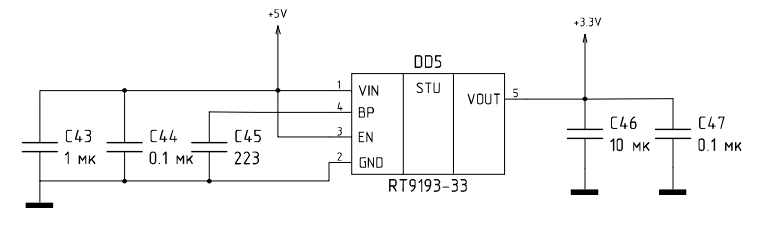
\includegraphics[width=0.4\textwidth]{images/design/mk_usb_stab}
    \caption{\centering Схема стабилизации питания МК-системы}
    \label{fig:mk_usb_stab}
\end{figure}

%\paragraph{Расчет сопротивления резисторов}

На принципиальной схеме расположено несколько резисторов.

Резистор R1 используется для стабилизации тока на источнике тактирования.
Резистор R2 используется для подтягивания линии RESET до 3.3 В.
Их номиналы установлены согласно документации на микроконтроллер\cite{stm32f103_datasheet}.

Резисторы R2--R5 добавлены для токоорганичния разъема USB, который используется для питания.

В Bluetooth-модуле, согласно документации, Резисторы R9, R6 имеют номинал 1 кОм и 220 кОм соответственно, а R7, R8~--- 10 кОм.

В состав NFC-модуля PN5180, согласно документации, входят резисторы R10, R13 сопротивлением 4.7 кОм и R11, R12, R14, R15 сопротивлением 2.2 кОм.

Дополнительно хотелось бы отметить, что расчет сопротивлений, емкостей и индуктивностей для PN5180 производился на основе раздела datasheet <<17.1 Typical component values>>\cite{pn5180_datasheet}.
В нем приведена схема с минимальным количеством компонентов и значения для них, представленные на рисунках~\ref{fig:pn5180mincomp} и~\ref{fig:pn5180mincompvalues} соответственно.


\begin{figure}[H]
    \centering
    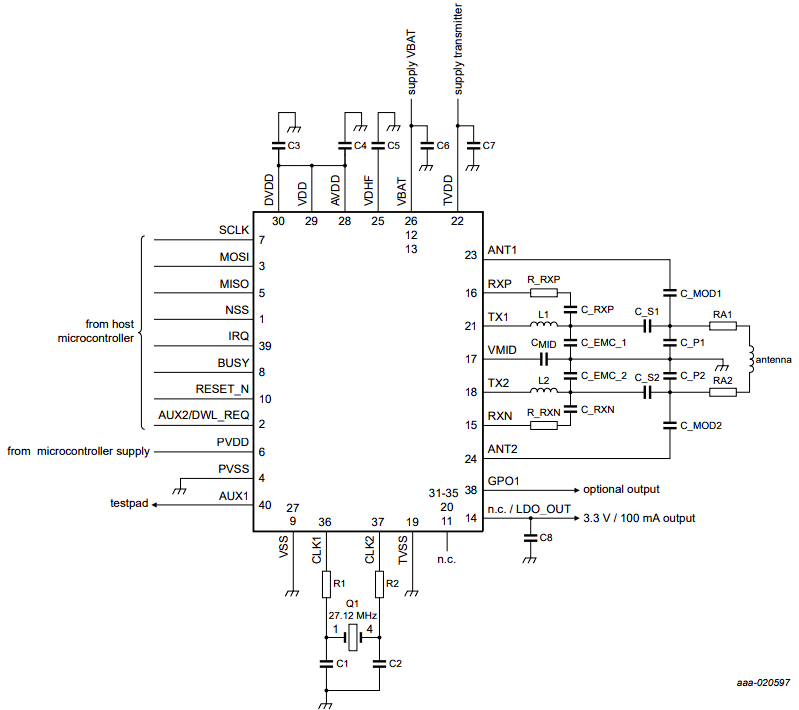
\includegraphics[width=0.7\textwidth]{images/design/pn5180mincomp}
    \caption{\centering Схема модуля PN5180 с минимальным набором элементов}
    \label{fig:pn5180mincomp}
\end{figure}


\begin{figure}[H]
    \centering
    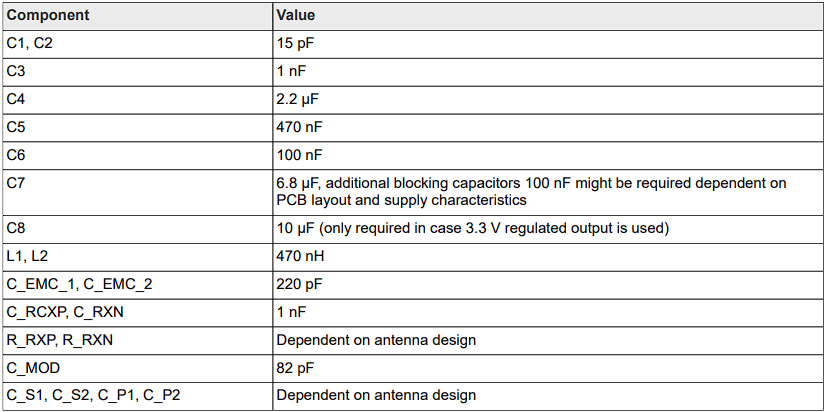
\includegraphics[width=0.7\textwidth]{images/design/pn5180mincompvalues}
    \caption{\centering Значения для элементов PN5180}
    \label{fig:pn5180mincompvalues}
\end{figure}

Также в открытом доступе находится принципиальная электрическая схема первой ревизии модуля PN5180 от производителя, которая и послужила основой для собственной электрической принципиальной схемы\cite{pn5180_schematic}.

% TODO: Подключение модулей

На основе всех вышеописанных сведений была спроектирована принципиальная схема разрабатываемой системы, показанная на рисунке~\ref{fig:principal_scheme} и в приложении Г.

\begin{figure}[H]
    \centering
    \fbox{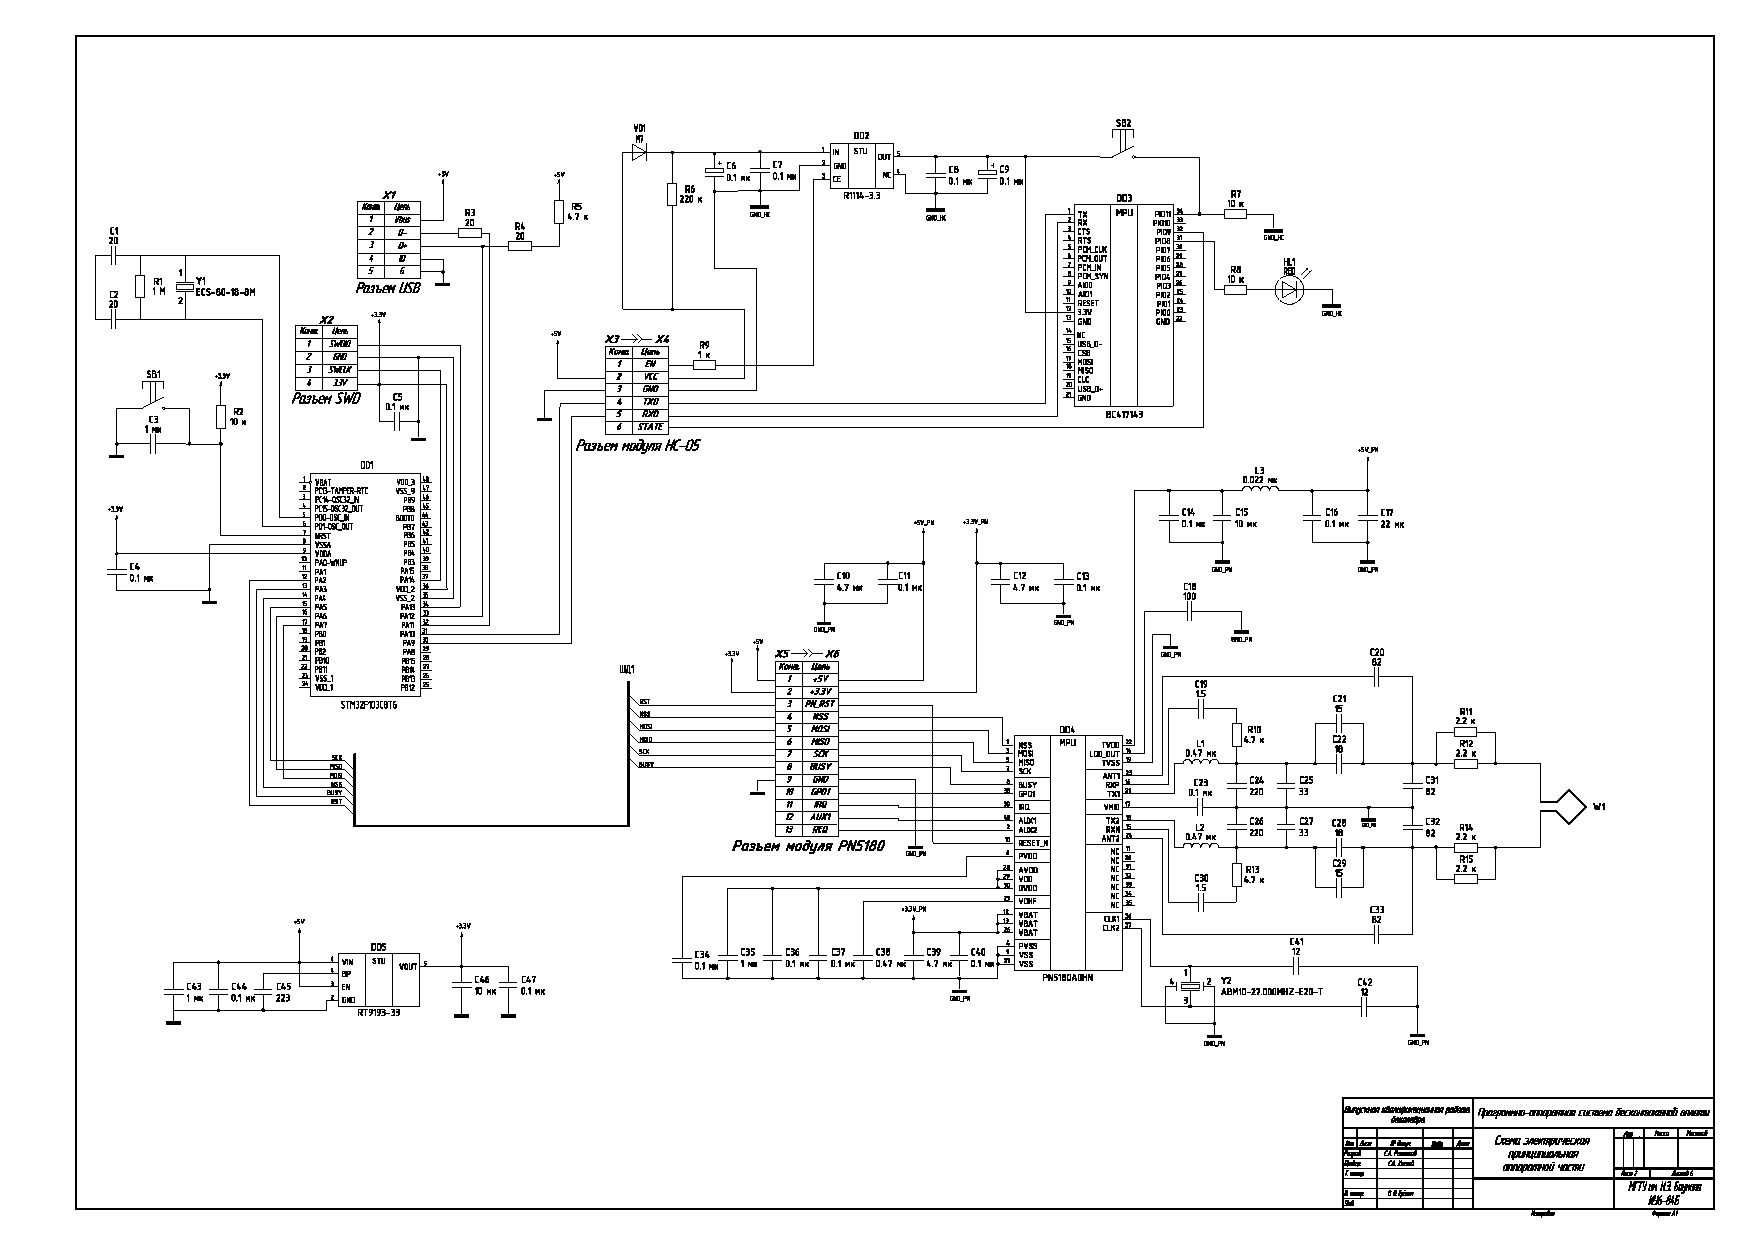
\includegraphics[angle=90, height=0.85\textheight]{appendices/schemas_princip.pdf}}
    \caption{\centering Схема электрическая принципиальная разрабатываемого устройства}
    \label{fig:principal_scheme}
\end{figure}





\subsubsection{Макет аппаратной части системы}

В качестве МК для макета используется STM32F103C8T6 в составе отладочной платы Blue Pill, представленной на рисунке~\ref{fig:blue_pill}.

\begin{figure}[H]
    \centering
    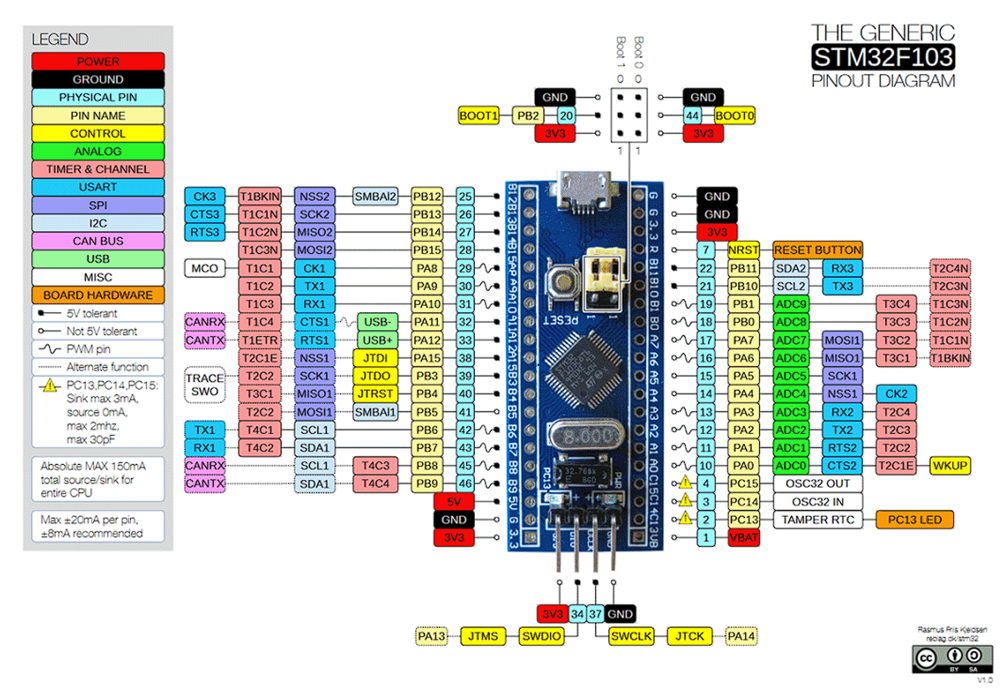
\includegraphics[width=0.8\textwidth]{images/design/blue_pill}
    \caption{\centering Отладочная плата Blue Pill с МК STM32F103C8T6}
    \label{fig:blue_pill}
\end{figure}

Сборка макета происходила в соответствии с принципиальной схемой с рисунка~\ref{fig:principal_scheme} и представлена на рисунке~\ref{fig:maket}.

\begin{figure}[H]
    \centering
    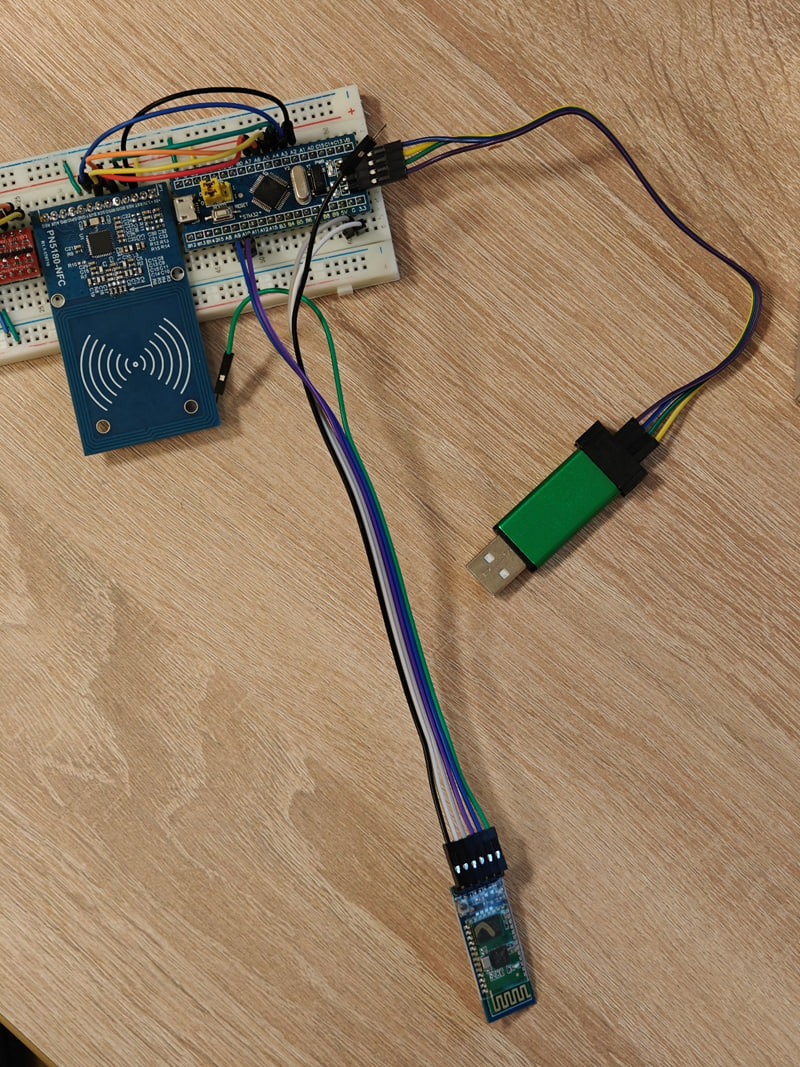
\includegraphics[width=0.5\textwidth]{images/design/maket}
    \caption{\centering Собранный макет устройства}
    \label{fig:maket}
\end{figure}

Для разработанного устройства-считывателя также был произведен расчет мощности.
Мощность, потребляемая разработанной схемой, складывается из мощностей, потребляемых всеми устройствами из ее состава.
Из документации используемых устройств получена информация, приведенная в таблице~\ref{tab:power}.
Расчет максимальной мощности, потребляемой устройством, определяется по формуле:

$$
P_{max} = \sum_{i=1}^{k} U_i \cdot I_{i_{max}} \cdot n_i
$$
где $U_i$~--- напряжение питания устройства, $I_{i_{max}}$~--- максимальный ток потребления, $n_i$~--- количество элементов в системе.

\begin{longtable}[l]{|
P{0.23\textwidth}|
P{0.15\textwidth}|
P{0.15\textwidth}|
P{0.15\textwidth}|
P{0.2\textwidth}|}

    \caption{Сравнение микросхем по потребляемой мощности}
    \label{tab:power} \\
    \hline
    \textbf{Микросхема} &
    \textbf{Ток потребления, мА} &
    \textbf{Потребляемая мощность, мВт} &
    \textbf{Количество устройств} &
    \textbf{Суммарная мощность, мВт} \\
    \hline
    \endfirsthead

    \caption*{Продолжение таблицы~\ref{tab:power}} \\
    \hline
    \textbf{Микросхема} &
    \textbf{Ток потребления, мА} &
    \textbf{Потребляемая мощность, мВт} &
    \textbf{Количество устройств} &
    \textbf{Суммарная мощность, мВт} \\
    \hline
    \endhead

    \hline
    \endfoot

    \hline
    \endlastfoot

    STM32F103\-C8T6 & 10 & 50 & 1 & 50 \\ \hline

    BC417143 & 70 & 231 & 1 & 231 \\ \hline

    PN5180A0NH & 20 & 60,6 & 1 & 60,6 \\ \hline

    R1114-3.3 & 100 & 500 & 1 & 500 \\ \hline

    CD1206-S01575 & 150 & 750 & 1 & 750 \\ \hline

    LP2985-33DBVR & 150 & 750 & 1 & 750 \\ \hline

    NCP1117-ST50T3G & 800 & 4500 & 1 & 4500 \\ \hline
\end{longtable}

При питании 5 В суммарная мощность системы будет приблизительно равна 6,342 Вт.

% TODO: make correct расчет потребляемой мощности


\subsection{Разработка программной части системы}

\subsubsection{Программа считывателя платежных средств}

% todo: добавить рисунок для mir

В основу алгоритмов работы устройства легли алгоритмы, представлены на рисунках~\ref{fig:pcd_flow} и~\ref{fig:pcd_flow_2_picc_activation},~\ref{fig:transaction_flow_example} и~\ref{fig:kernel_transaction_flow}, а также алгоритмы из спецификации для ПС <<МИР>>~\cite{book_mir}.
На основе них были разработаны несколько алгоритмов:

\begin{itemize}
    \item алгоритм перезагрузки NFC-модуля, представленный на рисунке~\ref{fig:restart_pn5180};
    \item алгоритм выполнения платежной транзакции, представленный на рисунке~\ref{fig:complete_transaction};
    \item алгоритм активации протокола ISO/IEC 14443--3, представленный на рисунке~\ref{fig:activate_iso3};
    \item алгоритм активации протокола ISO/IEC 14443--4, представленный на рисунке~\ref{fig:activate_iso4};
    \item алгоритм поиска платежных данных AFL, представленный на рисунке~\ref{fig:find_afl}.
\end{itemize}


\begin{figure}[H]
    \centering
    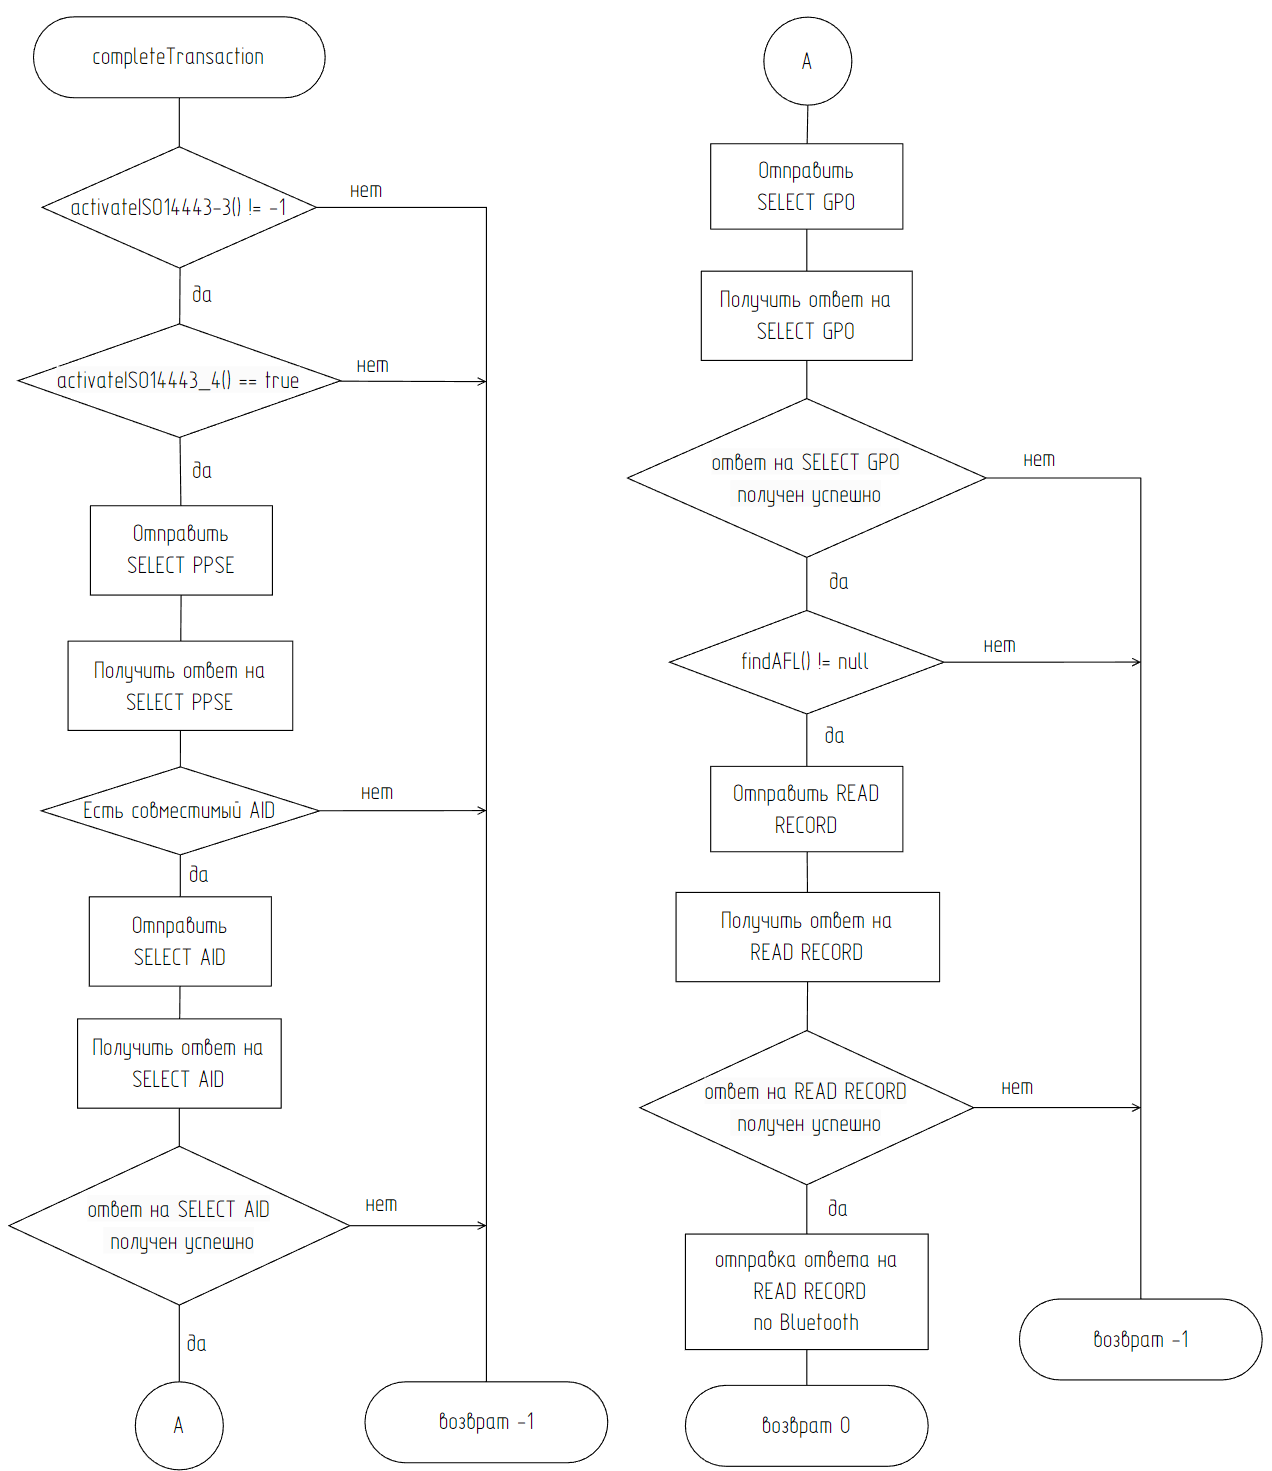
\includegraphics[width=0.9\textwidth]{images/design/complete_transaction}
    \caption{\centering Схема алгоритма выполнения платежной транзакции}
    \label{fig:complete_transaction}
\end{figure}

\begin{figure}[H]
    \centering
    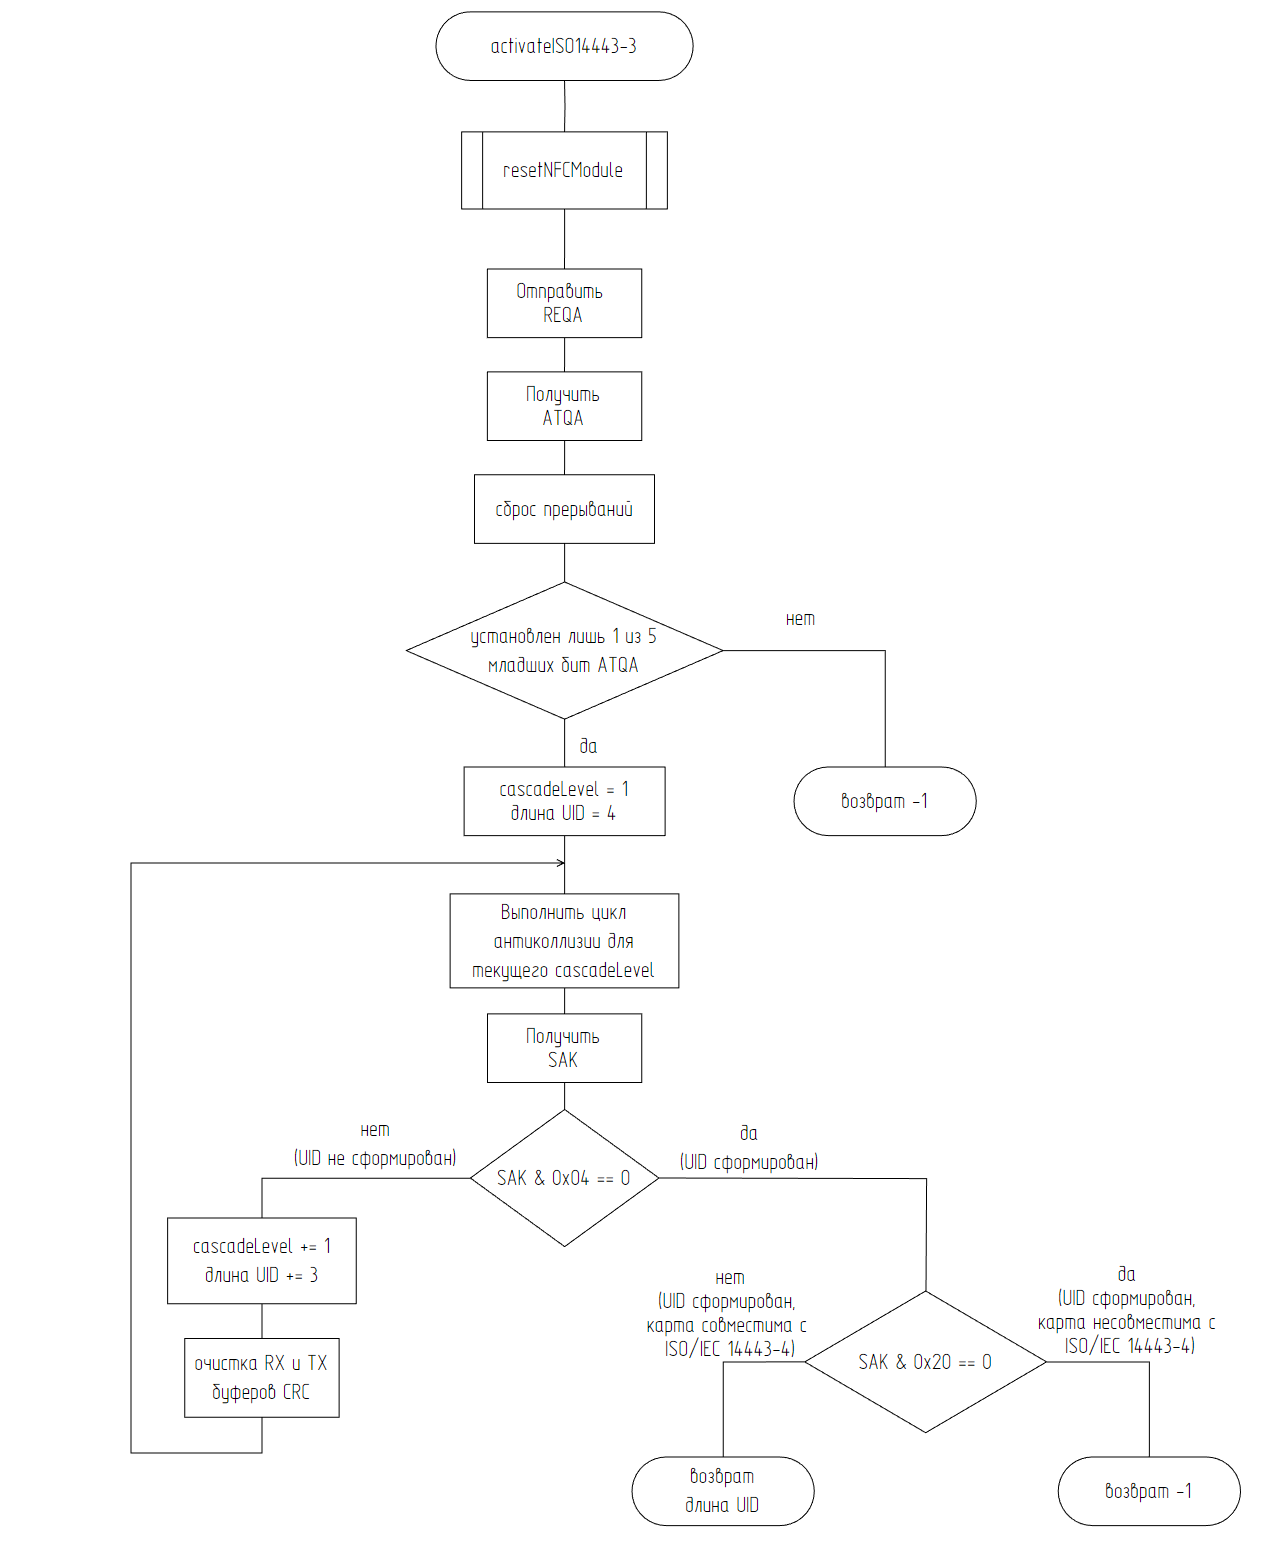
\includegraphics[width=0.8\textwidth]{images/design/activate_iso3}
    \caption{\centering Схема алгоритма активации протокола ISO/IEC 14443--3}
    \label{fig:activate_iso3}
\end{figure}

\begin{figure}[H]
    \centering
    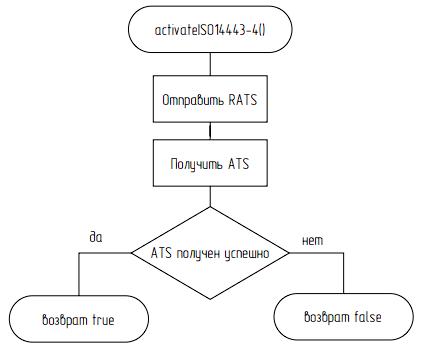
\includegraphics[width=0.5\textwidth]{images/design/activate_iso4}
    \caption{\centering Схема алгоритма активации протокола ISO/IEC 14443--4}
    \label{fig:activate_iso4}
\end{figure}

\begin{figure}[H]
    \centering
    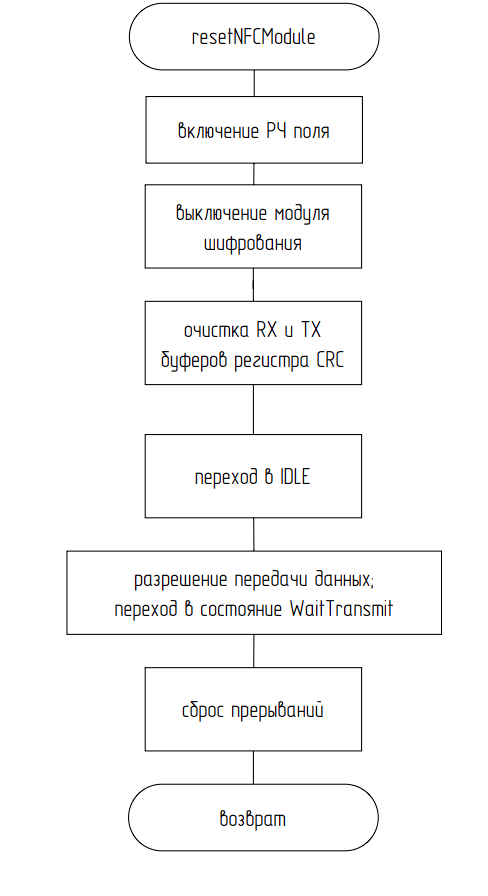
\includegraphics[width=0.3\textwidth]{images/design/restart_pn5180}
    \caption{\centering Схема алгоритма перезагрузки NFC-модуля}
    \label{fig:restart_pn5180}
\end{figure}

\begin{figure}[H]
    \centering
    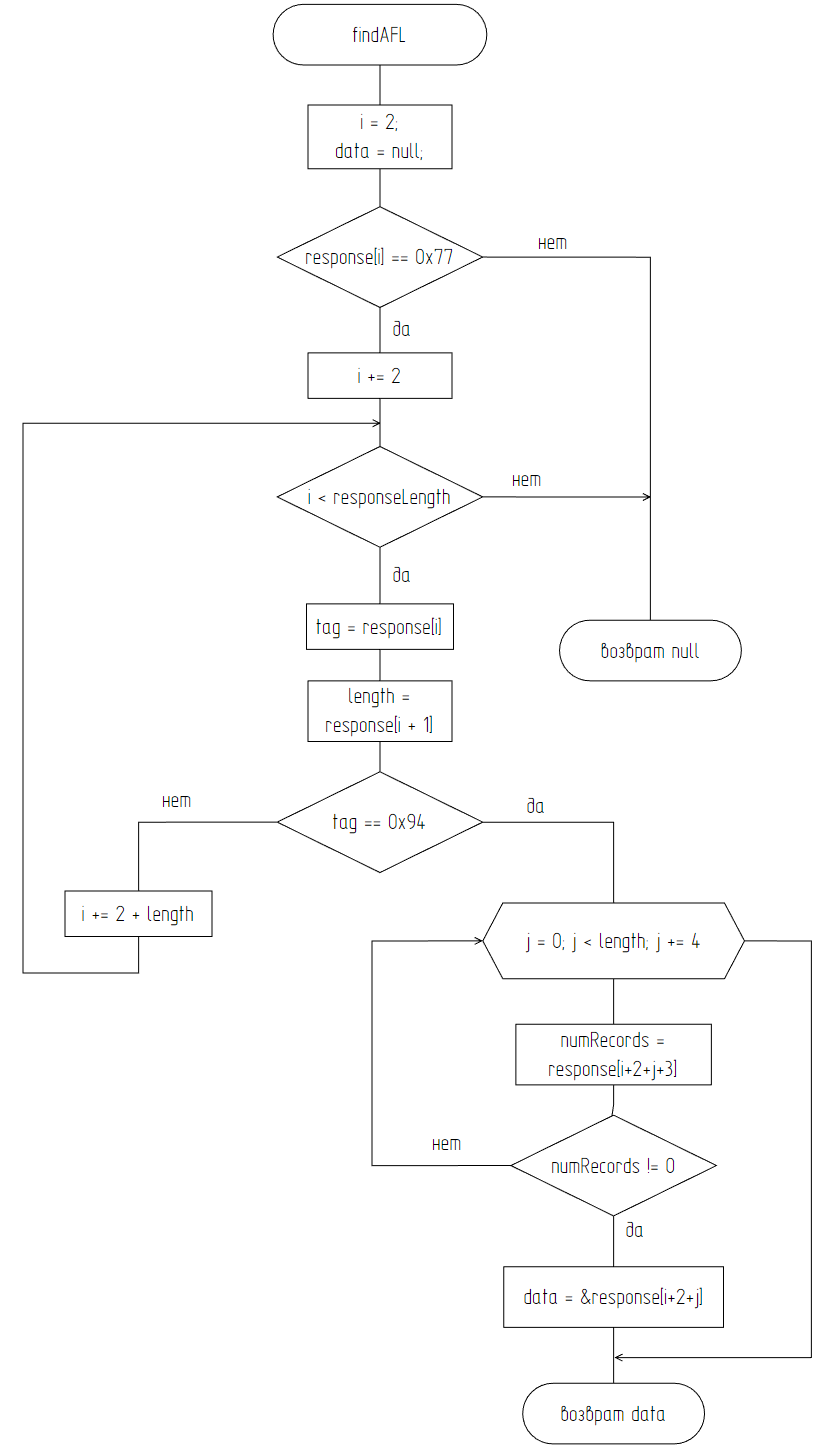
\includegraphics[width=0.6\textwidth]{images/design/find_afl}
    \caption{\centering Схема алгоритма поиска платежных данных AFL}
    \label{fig:find_afl}
\end{figure}


На рисунке~\ref{fig:find_afl} представлен алгоритм поиска значения тега Application File Locator, а точнее того, чтение которого является обязательным для активации транзакции, на это указывает numRecords != 0, если оно не равно 0, то эту запись нужно считать для транзакции (пояснение приведено на рисунке~\ref{fig:afl_pic}), в то время как для других записей в AFL данный тег установлен не будет.

\begin{figure}[H]
    \centering
    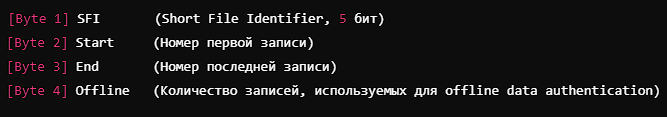
\includegraphics[width=0.7\textwidth]{images/design/afl_pic}
    \caption{\centering Формат кадра AFL}
    \label{fig:afl_pic}
\end{figure}

На основе найденного значения формируется запрос Read Record.
Правила формирования следующие:

\begin{itemize}
    \item CLA = 0x00  - класс команды,
    \item INS = 0xB2 - тип инструкции (Read Record),
    \item P1 = Start - индекс первого байта,
    \item P2 = SFI|4 - второй параметр команды на основе SFI,
    \item Lc = 0x00 - ожидаемое количество байт в ответе (0 - любое).
\end{itemize}

Разработка программного обеспечения устройства происходила в среде STM32CubeIDE, предназначенной для разработки на микроконтроллерах серии STM32.
STM32 умеет производить компиляцию с файлов C и C++ с помощью gcc и g++.
В качестве основного языка программирования использовался C++, т.к. в отличие от C он предоставляет широкую поддержку парадигмы объектно-ориентированного программирования.
Сама программа имеет модульный характер, на основе того, что в соответствие каждому аппаратному модулю (кроме МК) поставлен программный модуль, реализующий основные свойства и методы класса.

Настройка STM32F103C8T6 производилась с помощью графических средств STM32CubeIDE. Пример такой настройки является настройка источника тактирования, представленная на рисунке~\ref{fig:stm_cube}.

\begin{figure}[H]
    \centering
    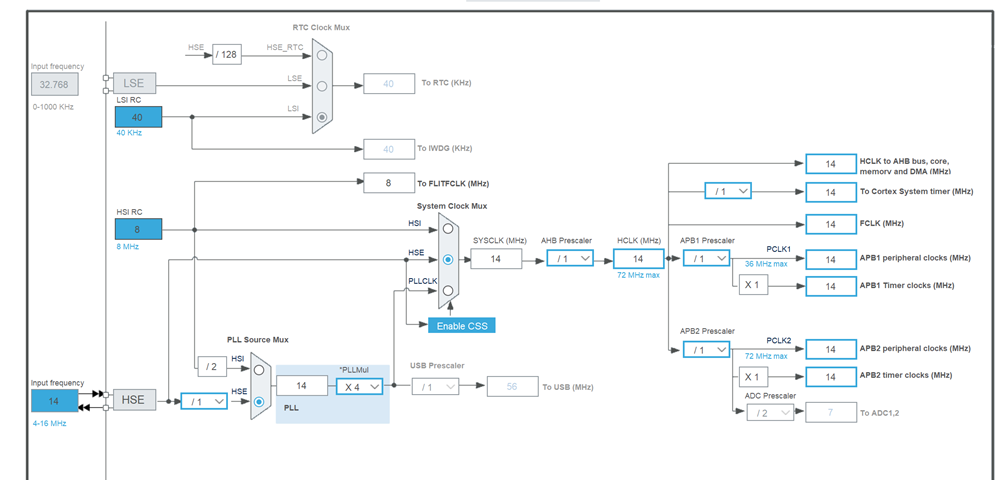
\includegraphics[width=0.9\textwidth]{images/design/stm_cube}
    \caption{\centering Настройка источника тактирования STM32F103C8T6}
    \label{fig:stm_cube}
\end{figure}

В качестве частоты используется 14 МГц для достижения максимальной скорости передачи данных с PN5180, который поддерживает максимальную скорость в 7 Мбит/с.
С помощью предделителя частоты SPI, равного 2, частота APB2 (именно к ней подключен SPI1) понижается до 7 МГц и 7 Мбит/с соответственно.
В приложении Б приведены листинги со следующими фрагментами кода:
\begin{itemize}
    \item настройка SPI для подключения PN51804
    \item настройка USART для подключения Bluetooth-модуля HC-05.
\end{itemize}

Взаимодействие с PN5180 разделено на два класса PN5180 и PN5180ISO14443.
Первый описывает реализацию основных методов управления состоянием модуля, а второй реализует специфичные для стандарта ISO14443 методы работы, с помощью которых осуществляется взаимодействие NFC-модуля и платежного средства.
Примеры процедур, реализующих их, также приведены в приложении Б.


\subsubsection{Программа мобильного устройства}
